\chapter{Background} \label{chap:Background}

\setcounter{secnumdepth}{3}
\renewcommand{\thesubsubsection}{\Alph{subsubsection}}

%\titleformat{\subsubsection}
%{\selectfont}{\thesubsubsection}{1em}{}

%Give background about polar codes and their adoption in 5G.

Polar codes were introduced by Arikan in his seminal work \cite{Arikan}. They belong to the class of capacity achieving codes. In the past decade, polar codes have sparked a interest from both academia and industry alike, resulting in significant research work in improving performance. The 5\textsuperscript{th} generation wireless systems (5G) standardization has adopted polar codes for uplink and downlink control information for the enhanced mobile broadband (eMBB). They are also considered as the potential coding schemes for two other frameworks of 5G, namely ultra-reliable-low-latency (URLLC) and massive machine-type communications (mMTC).

Polar codes achieve capacity asymptotically for memoryless channel. Although they are the first theoretically capacity achieving codes with an explicit construction, capacity is approached only asymptotically. Their performance is suboptimal compared to LDPC (Low Density Parity Check Codes) or Turbo codes at short block lengths with successive cancellation decoding (SCD). \cite{SCL} Presents the improved version of SCD called \emph{successive cancellation list decoder(SCLD)}.

The construction of polar codes involves the identification of channel reliability values. Information bits are placed in the K (number of information bits) high reliable bit indices out of N (block-length) positions and remaining bits are set to zero. These N bits are passed through a polar encoding circuit to get the encoded bits. Selection is of reliability indices is done based on the code length and channel signal-to-noise ratio. Due to varying code length and channel conditions in 5G systems, significant effort has been put to identify reliability indices which have good error correction performance over different code length and channel conditions.

\section{Background of Polar codes} 
This section introduces the basic mathematical foundations of the polar codes. In particular, about the frozen set design, encoding and decoding. Different decoding algorithms are introduced. Mainly Successive Cancellation (SC), Improved Successive Cancellation (fast-SSC) Successive Cancellation List(SCL). Examples of encoding and decoding with different algorithms are presented for better understanding.

%\subsection{Polar codes definition} \label{polarCodesDefn}

Mathematical foundations of polar codes lie on the polarization effect of the matrix \cite{Arikan}. $ k = \big[\begin{smallmatrix} 1 & 0 \\ 1 & 1 \end{smallmatrix}$\big] also called Arikan matrix. Polar codes are $(N,K)$ linear block codes of size $N = 2^{n}$ where $n$ being a natural number. $N$ is the block length of the code and $K$ is the number of information bits.  $N$-bit vector $U$ contains $K$ information and $N-K$ frozen bits which are set to known value mostly zeros. These bits are then multiplied with the generator matrix constructed from kronecker power\cite{kronecker} of Arikan kernel matrix.

For example $n=3$, block-length $N$ becomes $8$ hence the generator matrix is \newline

$ k^{\otimes 3} = \begin{bmatrix}
1 & 0 & 0 & 0 & 0 & 0 & 0 & 0\\ 
1 & 1 & 0 & 0 & 0 & 0 & 0 & 0\\ 
1 & 0 & 1 & 0 & 0 & 0 & 0 & 0\\ 
1 & 1 & 1 & 1 & 0 & 0 & 0 & 0\\ 
1 & 0 & 0 & 0 & 1 & 0 & 0 & 0\\ 
1 & 1 & 0 & 0 & 1 & 1 & 0 & 0\\ 
1 & 0 & 1 & 0 & 1 & 0 & 1 & 0\\ 
1 & 1 & 1 & 1 & 1 & 1 & 1 & 1
\end{bmatrix}$ \newline

where $k^{\otimes n}$ denotes the $n^{th}$ Kronecker power of $k$. The encoding process involves the multiplication of $N$-bit vector $U$ consisting of $K$ information bits and $N-K$ frozen bits with $k^{\otimes n}$.

\subsection{Polar code construction} \label{CodeConstruction}
In polar coding, first step is to identify the channel reliability values for a particular block length, this step is also called polar code construction. Basic idea  is to manufacture fraction of channels which are either completely noiseless or noisy out of $N$ (block-length) independent copies of given binary discrete memoryless channel. This process of creating extremal channels is called channel polarization. As $N\to\infty$, fraction of noiseless channels approaches the capacity of channel. Estimating reliability indices of channels is carried by considering the Bhattacharyya parameter\cite{Arikan}. Bhattacharyya parameter indicates the reliability of individual channel.
 
For a generic binary-input discrete memoryless channel (B-DMC) which is represented as $W \colon \mathcal{X} \to \mathcal{Y}$ with input alphabet $\mathcal{X}$, output alphabet $\mathcal{Y}$ and transition probabilities given by $W(y|x),x \in \mathcal{X}, y \in \mathcal{Y}$.

Bhattacharyya parameter is given by 
\begin{equation}
	Z(W) \triangleq \sum_{y \in \mathcal{Y}} \sqrt{W(y|0)W(y|1)}
\end{equation}

Bhattacharyya parameter indicates how unreliable the channel is, It is easy see that $Z(W)$ takes values between $[0,1]$ better the channel smaller is the $Z(W)$. Polarization creates channels with $Z(W)$ of 0 or 1.

\TODO{Here Give one example channel polarization for BEC channel and show the evolution of channel reliabilities. may be include a insert a picture with evolution of channel reliabilities plot. Does this make sense?}


\subsection{Encoding} \label{polarEncoding}
After polar code constructions, Out of $N$ bit positions information bits are placed in the most reliable bit indices position and non reliable bit positions are called frozen bits whose values are set to zero. This $N$-bit vector $U$ is multiplied with generator matrix obtained by the kronecker power of Arikan kernel matrix. Multiplying with generator matrix can also be represented as circuit form. Arikan kernel matrix can also be represented in circuit form as shown in figure \ref{fig:butterFlyCicuit} also called butter fly circuit.

\begin{figure}[h]
	\centering
	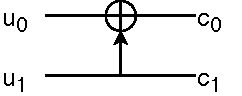
\includegraphics{./figures/ButterFlyCircuit.pdf}
	\caption{Butterfly circuit representing Arikan Kernel matrix}
	\label{fig:butterFlyCicuit}
\end{figure}

For $n = 3$ block length $N$ becomes 8 for such a case encoding circuit looks shown in  figure ~\ref{fig:encoderCircuit}, which is a repeated application of butter fly circuit. The read locations are the frozen bit indices which are set to zero, in remaining positions information bits are inserted. Output of the circuit is a code word which is transmitted over the channel. Lets consider an example with $N = 8$ and $K = 4$, rate of this code is $R = K/N = 1/2$. As given in the figure frozen bit indices are ${\{0,1,2,4\}}$ remaining indices contain information bits.  Let the information which needs to transmitted be \{1,1,0,0\}, then after placing information bits at reliable channel positions the vector $U$ becomes \{0,0,0,1,0,1,0,0\}. It is passed through the polar encoding circuit shown in Figure ~\ref{fig:encoderCircuit}. Result at the output of encoder is \{0,0,1,1,1,1,0,0\}. These encoded bits are then transmitted over the channel.

\begin{figure}[h]
	\centering
	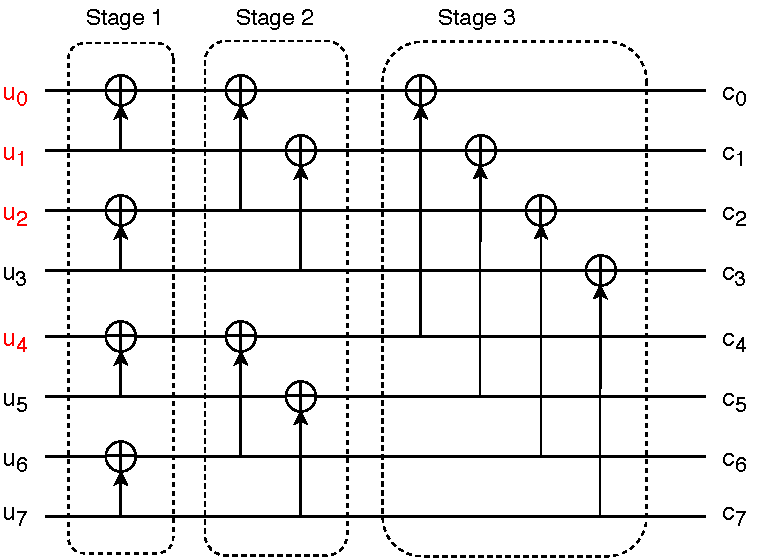
\includegraphics[width=0.8\textwidth]{./figures/EncodingCircuitStagesNew.pdf}
	\caption{Polar encoder in circuit form for $N = 8$}
	\label{fig:encoderCircuit}
\end{figure}

The encoding circuit is nothing but recursive application of the transformation represented by the butterfly circuit shown in the figure ~\ref{fig:butterFlyCicuit}. One butterfly unit can transform two uncorrelated bits $(a,b)$ into two correlated output bits $(a\oplus b,b)$ which is dominated by $k$ the Arikan Matrix. This corresponds to two channel polarization. In the above example reliability of the $u_{1}$ is increased compared to the $u_{0}$ channel. This operation recursively applied to the whole code word results in the circuit shown in the figure ~\ref{fig:encoderCircuit}. Code word splits into two parts in stage-3, which again splits into two parts in stage-2 and so on, until one reaches to single source bit $u_{i}$ in stage-1. So the process of polar encoding for $N = 8$ involves three stages of butterfly operations. Generally for a given code length $N=2^{n}$, the polar encoding consists of stages each with $N/2$ butterfly operations, which results in an encoding complexity of $O(N\log(N))$.


%\TODO{If you find any interesting, useful information for better understanding of the polar encoding, don't hesitate to include here.}

\subsection{Decoding}
As shown in section ~\ref{polarEncoding}, repetitive application of butterfly operation during encoding introduces correlation between the source bits. At the receiver, this is exploited to estimate the transmitted codeword. Utilizing the high correlation between the source bits forms the central idea behind the basic polar decoding algorithm called \emph{Successive Cancellation (SC)}. This method sequentially decodes each of the bits and takes previously estimated value to account for estimating the next bit. This sequential decoding exploits correlation between the source bits which as introduced during polar encoding process. Due to the sequential nature of SC decoding, the process has high. Improving the basic decoding algorithm has been the topic of researchers in academia and industry. These improvements are mainly directed towards two goals, first reducing decoding latency and second improving the error correction performance. Significant reduction in decoding latency is achieved by \cite{SSC} and \cite{fastSSC}. In these works, instead of decoding sequentially individual bit, special nodes are identified which can be decoded in parallel. Although polar codes are the first theoretically capacity achieving codes with explicit construction, their error correction performance at short block lengths is not comparable with that of LDPC or Turbo codes. This behavior can be better explained by the way decoding is performed. As presented earlier SC algorithm works by sequentially decoding individual bits and using information of previously decoded bits for estimating next bit. The issue with algorithm is if the previously decoded bit is wrong, then there is no way of correcting this bit.

To overcome this problem \cite{SCL} presents a improved version of the SC algorithm called Successive Cancellation List Decoding (SCL). The basic idea is instead of deciding a value of bit $u_{i}$ it takes both options, this results in two decoding paths for every bit, so to avoid exponential growth of complexity decoding candidates are restricted to $L$ the list size. At the end of decoding, most probable candidate is chosen from list. Performance of polar codes with SCL is still not as good as LDPC or Turbo codes at small and moderate block lengths. Polar code concatenated with CRC as outer code beats the LDPC codes of similar block length \cite{SCL}. SCL algorithm has a better error correction performance than SC, however it comes with a increased complexity and high decoding latency. Due to these reasons, in this work only fast-SSC algorithm is considered although its error correction performance is less than SCL.

\paragraph{\emph{A. Successive Cancellation Decoding (SC)}}  \label{SC}
The recursive SC decoder is basic algorithm presented in \cite{Arikan} for decoding polar codes.  SC decoder is inherently sequential, it estimates $\hat{u_{i}}$ of $u_{i}$ by using channel observation $y^{N}_{1}$ and all the previously decoded bits $\hat{u}_{1}^{i-1}$. If $u_{i}$ is frozen bit, the decoder assigns $\hat{u_{i}}$ to known value (mostly zero). If $u_{i}$ is an information bit, the decoder waits for all the previous bits to compute the decoding metric. It may be one of the three different type of metrics: \newline

$\bullet$ log-likelihood ratio (LLR) where


\begin{equation}
L_{N}^{(i)}(y_{1}^{N},\hat{u_{1}}^{i-1}) = \ln{\Bigg(\frac{W_{N}^{(i)}(y_{1}^{N},\hat{u_{1}}^{i-1}|u_{i} = 0)} {W_{N}^{(i)}(y_{1}^{N},\hat{u_{1}^{i-1}}|u_{i} = 1)}\Bigg)};
\end{equation}

$\bullet$ likelihood ratio (LR) where 

\begin{equation}
LR_{N}^{(i)}(y_{1}^{N},\hat{u_{1}}^{i-1}) = \Bigg(\frac{W_{N}^{(i)}(y_{1}^{N},\hat{u_{1}}^{i-1}|u_{i} = 0)} {W_{N}^{(i)}(y_{1}^{N},\hat{u_{1}^{i-1}}|u_{i} = 1)}\Bigg);
\end{equation}

$\bullet$ log-likelihood (LL) where 

\begin{equation}
LL(y_{1}^{N},\hat{u_{1}}^{i-1}) = \Big[ln\Big(W_{N}^{(i)}(y_{1}^{N},\hat{u_{1}}^{i-1}|u_{i} = 0)\Big), ln\Big(W_{N}^{(i)}(y_{1}^{N},\hat{u_{1}^{i-1}}|u_{i} = 1)\Big)\Big];
\end{equation}


Decoding metric computed from LLR's exhibit better numerical stability than those from LR's or LL's, so we have used the LLR's metric throughout this work. There are different ways to view and understand the operation of SC decoder. In this work decoding is viewed as message passing algorithm on an binary tree with $\log(N)$ levels. Decoding is performed by traversing a tree from root to leaf node. Process of decoding involves check node(CN), variable node (VN) operations and threshold detection at the leaf node. Decoder receives a LLR value for every bit which needs to be decoded (including both frozen and information bits), hence for a code with block length $N$, SC decoder receives $N$ LLR values. Decoding process estimates the bits $\hat{u}_{i} $  where $i = 0,1,2...,(N-1)$. The decoding tree for $N = 8$ looks as shown in the figure ~\ref{fig:decodingTree}.

\begin{figure}[h]
	\centering
	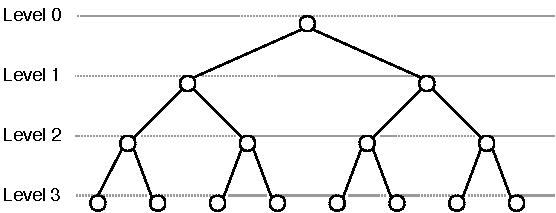
\includegraphics{./figures/decodingTree.pdf}
	\caption{Decoding tree}
	\label{fig:decodingTree}
\end{figure}

\begin{figure}[h]
	\centering
	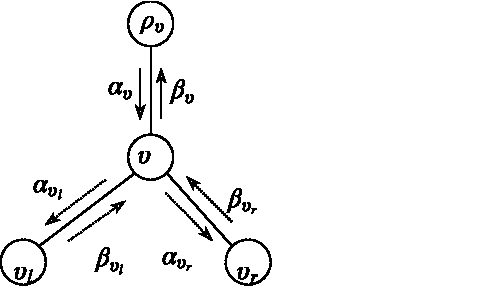
\includegraphics{./figures/messagePassingDiaS.pdf}
	\caption{Local Decoder}
	\label{fig:msgPassingDia}
\end{figure}

In a decoding  tree, the messages to left child node are computed with CN and to the right are with VN operation.  Figure ~\ref{fig:msgPassingDia} shows how the messages are exchanged in a local component decoder.

The CN and VN operations in LLR domain are given by following equations:

$\bullet$ Check Node (CN) operation

\begin{equation} \label{cnop}
	\alpha_{v_{l}}[i] = \alpha_{v}[i] + \alpha_{v}[i + N_{v}/2]
\end{equation}

$\bullet$ Variable Node (VN) operation

\begin{equation} \label{vnop}
\alpha_{v_{r}}[i] = \alpha_{v}[i + N_{v}/2] + (1 - 2\beta_{v_{l}}[i]) * \alpha_{v}[i]
\end{equation}

After decoding is done at both right and left child nodes the bits are combined at common parent node. the bit combining operation is given by the following equation.

\begin{equation*} \label{bitCombination}
\beta_{v}[i] = \begin{cases}
				\beta_{v_{l}}[i] \oplus \beta_{v_{r}}[i] & \text{if }i < N_{v}/2 \\
				\beta_{v_{r}}[i]
				\end{cases}
\end{equation*}

In the figure ~\ref{fig:msgPassingDia} and in equations ~\ref{cnop}, ~\ref{vnop}  $\alpha_{v}$, $\beta_{v}$ represent intermediate LLR values and estimated bits at the local decoder respectively.

Figure \ref{fig:scDecodingEg} gives an example of SC decoding for block-length $N=8$ and number of information bits $K=4$. In the figure decoded bits and intermediate $\beta_{v}$ are represented by black font color and computed intermediate $\alpha_{v}$ are indicated by green. Frozen pattern is provided below the leaf nodes. Frozen pattern indicates position of information and frozen bits. One in frozen pattern indicates frozen bit, zero indicates information bit.

\begin{figure}[h]
	\centering
	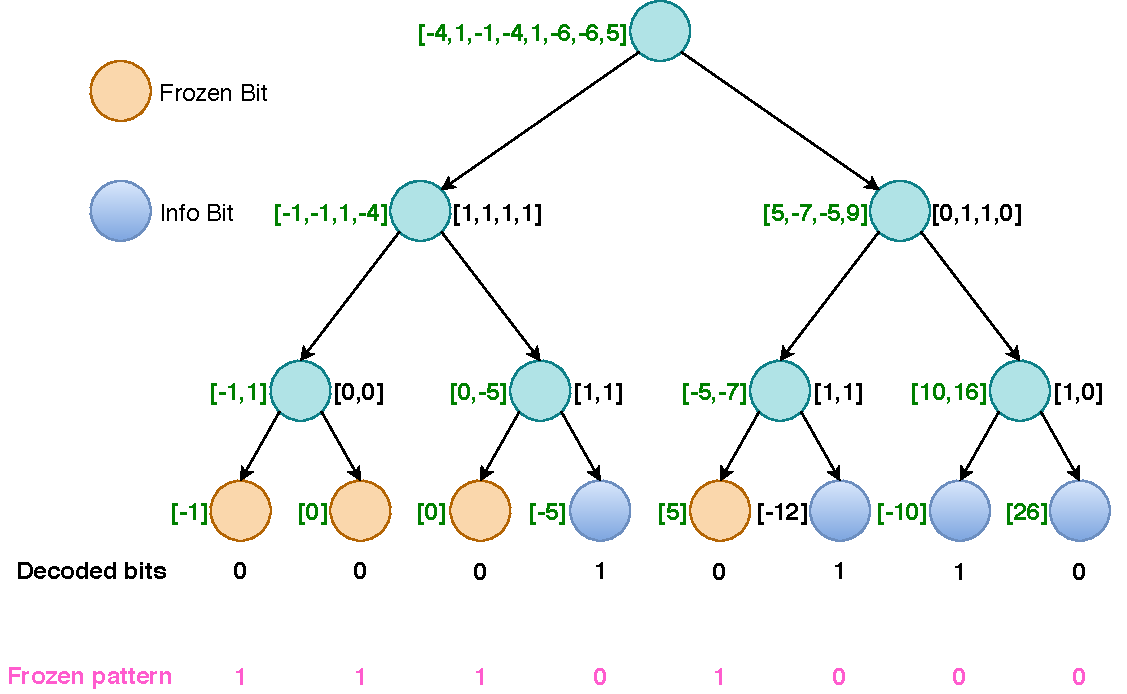
\includegraphics[width=0.9\textwidth]{./figures/SCDecodingExample.pdf}
	\caption{SC decoding example}
	\label{fig:scDecodingEg}
\end{figure}

%\TODO{provide an example of decoding with real LLR values for $N = 8$}

\paragraph{\emph{B. Improved Successive Cancellation Decoding (fast-SSC)}\newline}  \label{fastSSC} 
In basic SC algorithm, decoding is performed sequentially, previously decoded values are used for decoding the present bit. Due to sequential nature of the decoder, decoding latency is high.\cite{SSC} and \cite{fastSSC} try to identify special kind of nodes in a decoder tree which can be immediately decoded without traversing till the end of the tree. \cite{SSC} tries to identify node with all information bits or all frozen bits. These nodes are called rate-one($R1$) and rate-zero ($R0$) nodes respectively. The $R1$ node can be decoded by taking hard decision and polar transform, since there is no extra information which can be gained from traversing the tree. Decoding of $R0$ node is not necessary since none of them are information bits, so all the bits are set known value which is known at transmitter and receiver which are mostly set to zero. \par Authors in \cite{fastSSC} extend the idea presented in \cite{SSC} by identifying two more kind of special nodes which can be decoded without traversing the tree single parity check ($SPC$) and repetition ($REP$) nodes. Both in \cite{SSC} and \cite{fastSSC} node type is identified based on the frozen pattern at the component decoder. For $SPC$ node, only one frozen bit is present at left most position. For $REP$ node, frozen pattern contains one information bit at right most position, remaining are frozen bits.

One such example, when frozen indices for $N = 8$ are $\{0,1,3,4\}$. The full decoding tree of Figure ~\ref{fig:decodingTree} gets reduced to a tree with fewer nodes as shown in Figure ~\ref{fig:decodingTreePruned}. We can easily see that, in the original decoder tree number of nodes were $15$, in the pruned tree nodes are reduced to 7, which results in a significant reduction in number of computations and decoding latency.

\begin{figure}[h]
%	\centering
	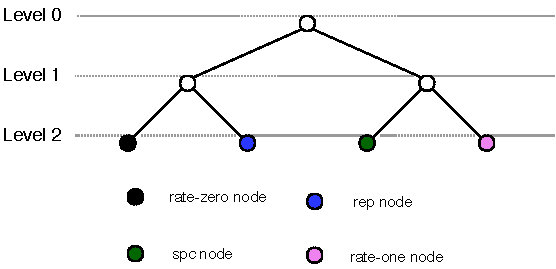
\includegraphics{./figures/decodingTreePruned.pdf}
	\caption{Pruned Decoder Tree}
	\label{fig:decodingTreePruned}
\end{figure}


%\paragraph{\emph{C. List Decoding of Polar Codes (SCL)}\newline}  \label{SCL}


%Here I need to explain the typical features which are important for understanding the latency contributors and how they can be resolved
\section{Processor architecture background}
To better understand the bottlenecks and optimizations performed in software implementation of 5G FEC chain, it is necessary to understand the fundamentals of processor architecture. This section gives necessary background about cache memory systems, instruction pipelining, branch predictors, Vector processing units and recursive function calling mechanism.

\subsection{Cache memory} \label{cacheSection}
In the modern processors, fast memory called cache is used to reduce the average access time of main memory also called RAM (Random Access Memory). Cache minimizes the number of accesses to RAM by storing frequently accessed location's data in it, hence avoiding huge penalty of reading data frequently from RAM which operates at a much lower frequency than the CPU. When memory location is accessed for the first time it is copied from RAM to cache, future accesses to same location is done via cache. These fast memory is placed between RAM and processor. In modern processors instead of single cache, multi-level caches are present. The main idea behind having multi-level caches is that if the data is not found in first level then second level is checked if not then third level until the last level, still if the data is not found then RAM is accessed. This model significantly reduces the probability of accessing the RAM compared to having a single level cache. Complete memory hierarchy of the modern processors is shown in the figure  ~\ref{fig:memoryHierarchy} \cite{CMP}.

\begin{figure}[h]
	\centering
	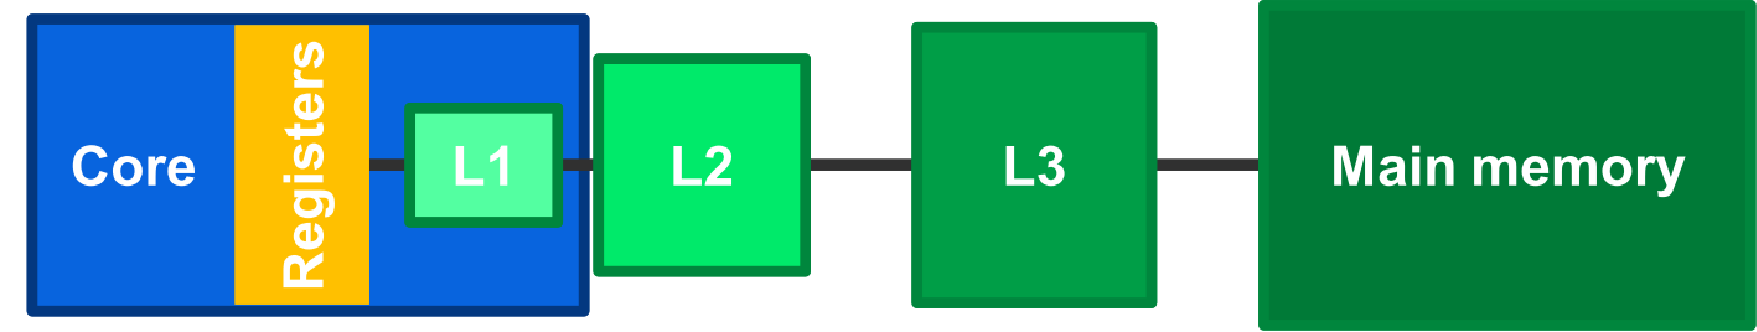
\includegraphics[width=0.7\textwidth]{./figures/memoryHierarchy.pdf}
	\caption{Memory Hierarchy}
	\label{fig:memoryHierarchy}
\end{figure}

Above figure shows processor architecture with three level caches namely L1, L2 and L3. In the order of increasing access latency, reducing cost and increasing size. L1 cache is fastest, costliest and smallest among all caches. Data is mapped to either memory or registers. If the available registers are not enough in such a case data is stored in memory. If the data is not found in all cache levels then it results in cache miss which causes processor instruction execution to stop until data is fetched from RAM. Whenever the memory location is accessed for the first time it always results in cache miss. Present data modern processors provide special instructions to avoid these compulsory cache misses, these are called cache prefetch instructions which allow programmer to fetch data from cache before it is accessed, hence hiding the memory access latency. Some other software techniques to reduce cache misses are reusing the allocated memory as much as possible and bit packing/unpacking to reduce the required memory. In this work, all the above mentioned techniques namely using prefetch instructions ($\mathtt{PREFETCH}$) provided by AMD EPYC processor, reusing the allocated memory and bit packing/unpacking are used reduce the memory access latency.

\subsection{Instruction pipelining and branch predictors}
Traditionally processors were designed to follow the steps fetch, decode, execute, memory finally write-back and then fetch the next instruction. Although these steps are sufficient to solve any problem in hand, it is very inefficient in terms of hardware utilization. When instruction is getting fetched, remaining modules are idle, if instruction is in decode phase remaining modules are idle similarly other phases. To overcome under utilization of hardware resources modern processors implement instruction pipelining concept, where if the current instruction is in decoding phase the next instruction will be concurrently fetched by the fetch module. Pipelining mechanism increases the instruction throughput by significantly reducing CPI (Cycles per Instruction). Example of sequential and pipelined execution is shown in figure \ref{fig:pipeline} \cite{SoCT}.

\begin{figure}[h]
	\centering
	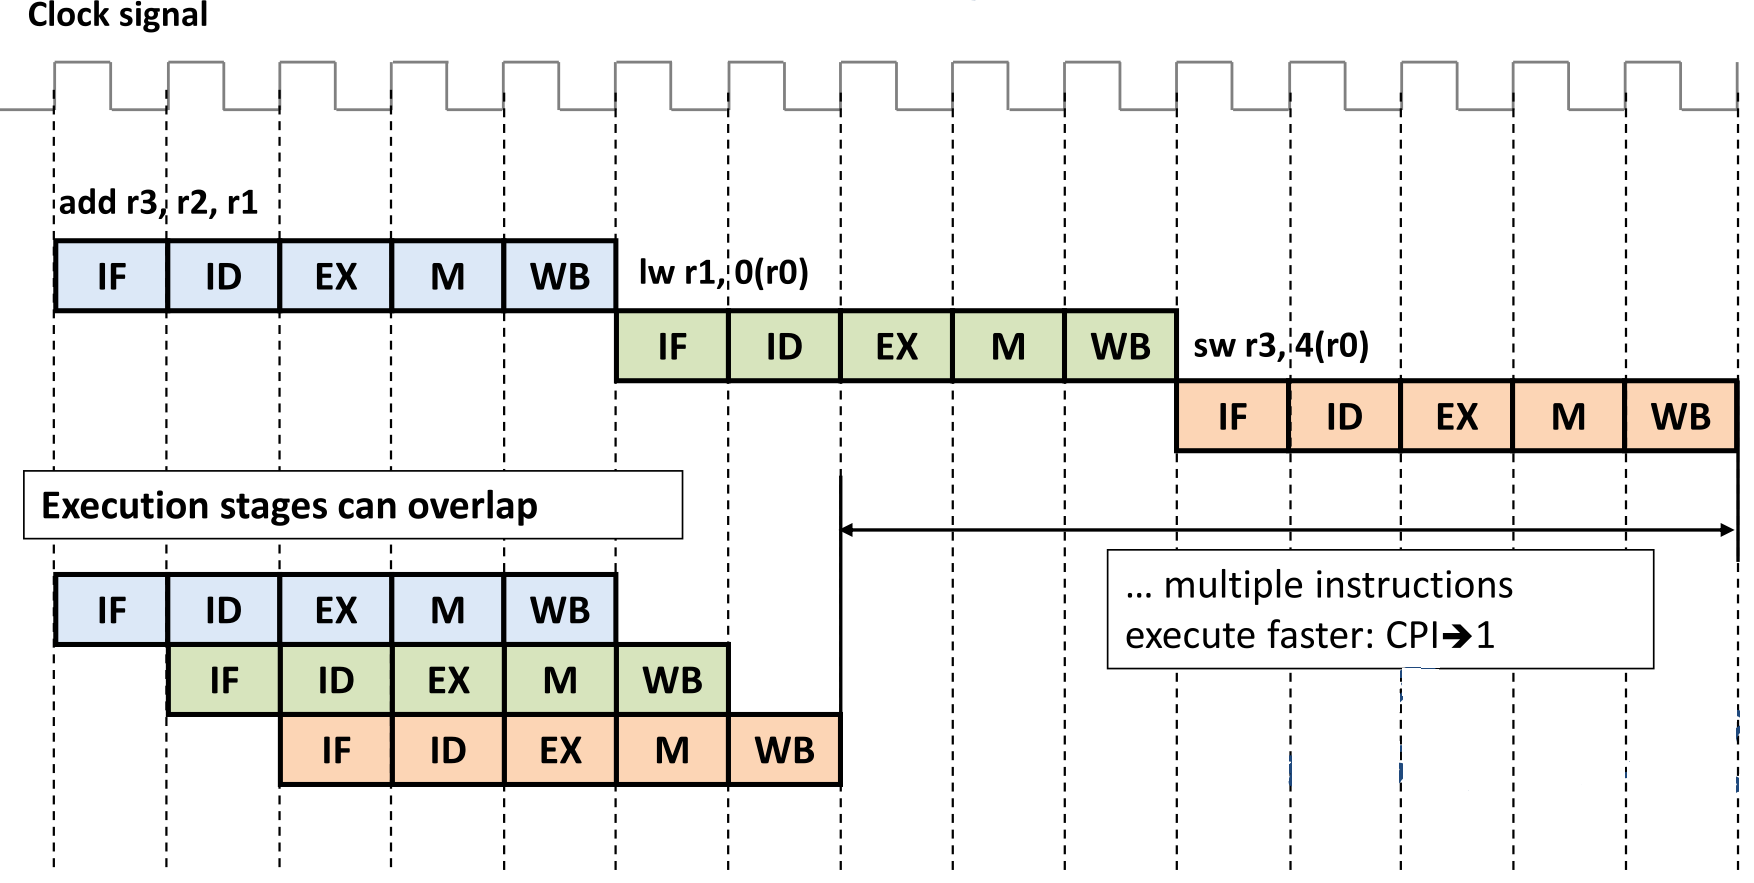
\includegraphics[width=0.9\textwidth]{./figures/pipeline_seq2_edited.pdf}
	\caption{Instruction pipelining}
	\label{fig:pipeline}
\end{figure}

Example shown in figure \ref{fig:pipeline} assumes only five phases of instruction execution. Modern processors divide instructions execution to nineteen plus phases, which allows running processor at much higher frequency due to reduced critical path delay. Maximum advantage of pipelining can only be exploited when there are no pipeline stalling or flushing which happen when there is a data dependency, cache misses or branch instructions. Major contributors to pipeline stalling are cache misses and branch instructions. As explained in \ref{cacheSection} can be reduced by using combination of different optimization techniques. Next culprit is branch instructions, whether to branch or not is decided only the at execution stage. By the time branching is decided, many of the future instructions are already fetched, if the decision is to jump then all the prefetched instructions must be flushed which introduces stall in the pipeline. To overcome this issue branch predictors are designed to pro-actively fetch instructions from correct address, hence avoiding flushing of pipeline. Branch predictors function by storing the previous decisions on the branching whether it was taken or not, hence requires correct previous state to pro actively fetch future instructions. This method reduces the pipeline caused due to looping type of code, by reducing pipeline flushes. For the scenarios where there are no looping instruction just if or if-else constructs branch predictors fail to correctly fetch the future instructions. These kind of scenarios can be minimized by avoiding branch instructions wherever possible and by providing hints to compiler built-in macros to reduce the branching by better placement of assembly instructions (kind of instruction scheduling). One such macro is 
\begin{minted}{c++}
	long __builtin_expect(long EXP, long C); 
\end{minted}
which tells compiler to place more frequently executing part of the code just after branch instruction to minimize pipeline flushing. Code snippet \ref{code:likelyHint} shows the typical usage.

\begin{code}
	\captionof{listing}{Branching hints to compiler}
	\label{code:likelyHint}
\begin{minted}{c++}
#define likely(expr) __builtin_expect(!!(expr), 1)
if (likely(a > 1)) {
	//Frequently executing part, most of the cases a is greater than 1
	...
} else {
	//Rarely executing part, rarely a is less than 1
	...
}
\end{minted}
\end{code}

Another feature provided by modern processors is conditional move instruction ($\mathtt{CMOV}$). Compiler intelligently maps if statements to conditional move instructions. $\mathtt{CMOV}$ copies a particular value to register or memory based on the flags set. It is not vulnerable to branch-prediction failure since no branch instructions gets generated, hence avoiding pipeline flushing. Following listing in \ref{code:NaiveCMOVEg} and \ref{code:CMOVEEg} illustrates the feature.

\begin{code}
	\captionof{listing}{Naive method}
	\label{code:NaiveCMOVEg}
\begin{minted}{c++}
uint32_t bitMask = 0;
if(CRCLENGTH == 6) //If Crc6 needs be calculated, then change the mask.
  bitMask = 0x3F;
else
  bitMask = 0x7FF;
\end{minted}
\end{code}

\begin{code}
	\captionof{listing}{With $\mathtt{CMOV}$}
	\label{code:CMOVEEg}
\begin{minted}{c++}
uint32_t bitMask = 0x7FF; //Initializing with CRC11 mask.
if(CRCLENGTH == 6) //If Crc6 needs be calculated, then change the mask.
  bitMask = 0x3F;
\end{minted}
\end{code}

Both code achieve same results, however \ref{code:NaiveCMOVEg} pipeline flush will happen due to branch-misprediction, for \ref{code:CMOVEEg} compiler identifies conditional move construct and generates $\mathtt{CMOV}$ potentially avoiding pipeline flush. Optimizations such as minimizing branches, using built-in macros and using constructs which help compiler to identify pattern are utilized in this work.

\subsection{Vector processing units}
Vector processing units are special kind of multiple computational elements that perform same operation on multiple data points simultaneously. Machines with vector processing units exploits data level parallelism but not concurrency. Same instruction operates on multiple data points in other words there are simultaneous computations but there is a single process. These special kind of instructions are also called SIMD (Single Instruction Multiple Data) in Flynn's taxonomy of parallel computers. These instructions are particularly useful when same operation needs to applied set of data, for example scaling a vector by constant. SIMD units can be thought of same processing unit replicated multiple times which are operated by a single instruction. Figure \ref{fig:simdUnits} from wikipedia \cite{SIMDWiki} illustrates the concept of SIMD and how single instruction pool operates on multiple data points.

\begin{figure}[h]
	\centering
	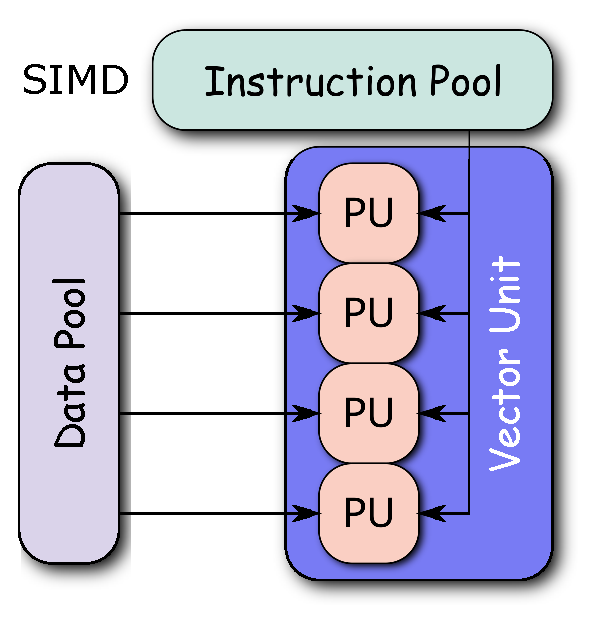
\includegraphics[width=0.5\textwidth]{./figures/SIMD2.eps}
	\caption{Vector processing units}
	\label{fig:simdUnits}
\end{figure}

Modern x86 processors from AMD and Intel provide different SIMD extensions named SSE (Streaming SIMD Extensions), AVX (Advanced Vector Extensions) with register size of 128-bits, AVX2(Advanced Vector Extensions 2) with register size 256-bits and the latest AVX-512 with register size 512-bits. In this work AMD EPYC processor used which provides SSE, AVX and AVX2 instructions, implementation is carried out using the features available in these extensions.

\subsection{Recursive function calling mechanism}
Most of the encoder and decoder implementations are implemented through recursion. Recursive function is a method which calls itself. It is a powerful tool in computer science which can be used for solving many interesting problems. However when it comes to performance, recursive problem solving falls behind algorithms which use looping to solve the same problem. Mainly due to the fact that every time a recursive function is called new stack frame is allocated, local data is pushed to call stack and execution must branch to the beginning of function. Branching and pushing data to call stack are expensive operations. In case of polar codes both encoding and decoding are implemented as recursive functions. To reduce the latency of FEC chain encoding/decoding implementations are unrolled to avoid recursions. For encoder, unrolling is carried out by manually implementing multiple inline functions. In decoder implementation unrolling is carried out by using C++ template concept. Although unrolling increases code size, for the application in hand latency is of at most importance than code size. Unrolling of the encoder and decoder implementations significantly improved the latency of FEC chain.